\chapter{软件设计实现}\label{chap:software}

\section{NVDLA 软件工具链概述}

在前面的章节,我们略微提到过 NVDLA 的软件栈。但是在这一小节,我们将详细的介绍 NVDLA 的软件工具链。如图~\ref{fig:NVDLA Software},英伟达官方提供了完整的软件生态。

\begin{figure}[!htbp]
    \centering
    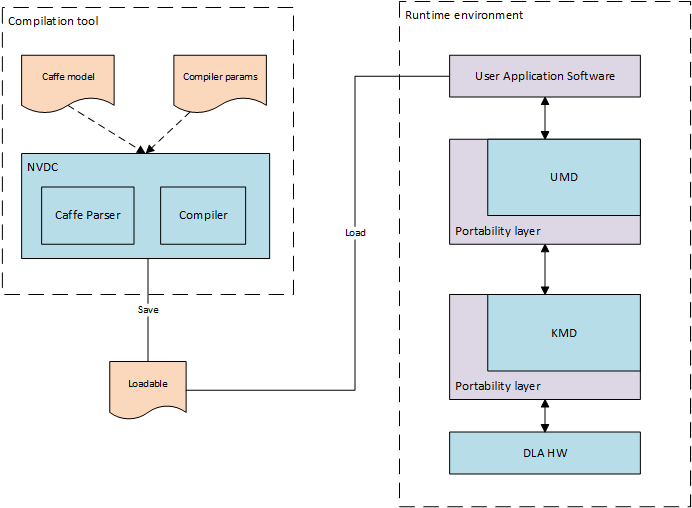
\includegraphics[width=0.7\textwidth]{software_package.png}
    \caption{NVDLA Software}
    \label{fig:NVDLA Software}
\end{figure}

Compiler 是软件工具链的前端,与硬件无关,Compiler 能够接受的参数如下:

\lstset{language=Bash}
\begin{lstlisting}
./nvdla_compiler -h
Usage: ./nvdla_compiler [-options] --prototxt <prototxt_file> --caffemodel <caffemodel_file>
where options include:
    -h                                                 print this help message
    -o <outputpath>                                    outputs wisdom files in 'outputpath' directory
    --profile <basic|default|performance|fast-math>    computation profile(fast-math by default)
    --cprecision <fp16|int8>                           compute precision(fp16 by default)
    --configtarget <nv_full|nv_large|nv_small>         target platform(opendla-full by default)
    --calibtable <int8 calib file>                     calibration table for INT8 networks
    --quantizationMode <per-kernel|per-filter>         quantization mode for INT8(per-kernel by default)

\end{lstlisting}

最终,Compiler 生成 Loadable 文件,交给 Runtime 进行加速器的调度。

Loadable 文件是 Compiler 与 Runtime 之间通信的媒介,其由 Google 开源的 FlatBuffers 序列化协议所组织,能够将对象与数据进行压缩,以便在网络中进行传输。简单来讲,我们需要在流中传输一个对象,比如网络流。一般我们需要把这个对象序列化之后才能在流中传输(例如,可以把对象直接转化为字符串),然后在接收端进行反序列化(例如把字符串解析成对象)。但是显然把对象转成字符串传输的方法效率十分低下,于是有了各种流的转换协议,FlatBuffers也是其中一种。

Runtime 与硬件紧密贴合,其又分为 UMD 和 KMD 两个部分:UMD 是用户应用,需要我们在 Linux 上编译运行,其接受 Loadable 文件并解析,最后递交一个推理任务到 KMD;KMD 是内核驱动,需要我们在构建 Linux 的时候编译,运行 Linux 的时候挂载,接受推理任务之后负责调度网络,配置寄存器,处理中断等任务。Runtime 能够接受的参数如下:

\lstset{language=Bash}
\begin{lstlisting}
./nvdla_runtime -h
Usage: ./nvdla_runtime [-options] --loadable <loadable_file>
where options include:
    -h                    print this help message
    -s                    launch test in server mode
    --image <file>        input jpg/pgm file
    --normalize <value>   normalize value for input image
    --mean <value>        comma separated mean value for input image
    --rawdump             dump raw dimg data

\end{lstlisting}

Compiler 的编译过程较简单,本设计不多介绍,Runtime 的编译过程非常复杂,将在后面的章节详细介绍。

\section{TensorRT 与模型量化}

本设计使用的 small 配置,仅支持 INT8 推理,而 Caffe 框架天生仅支持 Float32 类型的训练,所以我们需要进行模型的量化。

\section{Petalinux 工具介绍}


\section{Ubuntu 16.04 根文件系统移植}

\subsection{读取 Block Design 配置信息}

\subsection{Linux 内核裁剪}

\subsection{新增 Linux 设备树节点}

\subsection{生成 Boot 和 Image 文件}

\subsection{替换根文件系统}

\section{KMD 内核程序挂载}

\section{UMD 应用程序编译}
